\documentclass[a4paper, 11pt]{exam}
\usepackage[T1]{fontenc}
\usepackage{titling}
\usepackage{url}
\usepackage{amsmath,amsthm,amssymb}
\usepackage{graphicx}
\usepackage{graphics}
\usepackage{listings}
\usepackage[dvipsnames]{xcolor}
\usepackage{tabularx}
\usepackage{ragged2e}
\usepackage{courier}
\usepackage{textcomp}
\usepackage{circuitikz}
\usepackage{tikz}
\usepackage{enumitem }
\usepackage{karnaugh-map}
\usepackage{bytefield}
\usepackage{mathrsfs}
\usepackage{cancel}
\usepackage[linesnumbered,ruled,vlined]{algorithm2e}
\usepackage{hyperref}

\newcommand{\invlaplace}[1]{%
\mathscr{L}^{-1}\left\{#1\right\}
}
\newcommand{\laplace}[1]{%
\mathscr{L}\left\{#1\right\}
}
\newcommand{\fourier}[1]{%
\mathscr{F}\left\{#1\right\}
}

\newcommand{\ztransform}[1]{%
\mathscr{Z}\left\{#1\right\}
}

\newcommand{\subtitle}[1]{%
  \posttitle{%
    \par\end{center}
    \begin{center}\large#1\end{center}
    }%
}

\usepackage{environ}

\NewEnviron{eqnsection}[2]{%
  \newcommand{\myvspace}{#1}%
  \vspace{\myvspace}%
  \begin{align*}
  \intertext{#2}
  \BODY
  \end{align*}%
  \vspace{\myvspace}%
}


\newcommand{\uparrowat}[1]{\underset{\uparrow}{#1}}


\newlist{myenumerate}{enumerate}{2}
\setlist[myenumerate,1]{label=\roman*)}
\setlist[myenumerate,2]{label=\alph*)}



\newcommand\tab[1][1cm]{\hspace*{#1}}

\renewcommand{\labelenumi}{\alph{enumi})}

\title{Homework Assignment \#2}
\subtitle{ECE 6530: Digital Signal Processing \\
\today\\}
\author{ Miguel Gomez U1318856\\
\textbf{Homework set \#2}}
\date{Due Date: Sep 14, 2023\\
(100 points)}

\begin{document}
\maketitle
\noindent
\section{}
2.7 - Answer subquestions (1) through (5) for parts (a) through (e). (10 points)
\vspace{2em}
\hrule
\begin{enumerate}
\item $y(n) = \cos{(x(n))}$
\item $y(n) = \sum_{k=-\infty}^{n+1} x(k)$
\item $y(n) = x(n)\cos{(\omega_0n)}$
\item $y(n) = x(-n + 2)$
\item $y(n) = $Trun$[x(n)]$ where Trun$[x(n)]$ denotes the integer part of $x(n)$, obtained
by \\ truncation.
\end{enumerate}
\section{}
2.11 - Problem 2.11 (10 points)
\begin{eqnsection}{3em}{The following input–output pairs have been observed during the operation of a linear system:}
  x_1 (n) &= \lbrace-1, \uparrowat{2}, 1\rbrace \quad \overset{\text{$\mathcal{T}$}}{\longleftrightarrow}\quad y_1(n)=\lbrace1,\uparrowat{2},-1,0,1\rbrace \\
  x_2 (n) &= \lbrace−1, \uparrowat{-1}, -1\rbrace \quad \overset{\text{$\mathcal{T}$}}{\longleftrightarrow}\quad y_2(n)=\lbrace-1,\uparrowat{1},0,2\rbrace \\
  x_3 (n) &= \lbrace0, \uparrowat{1}, 1\rbrace \quad \overset{\text{$\mathcal{T}$}}{\longleftrightarrow}\quad y_3(n)=\lbrace\uparrowat{1},2,1\rbrace \\
   \intertext{Can we draw any conclusions regarding the linearity of the system. What is the impulse response of the system?}
 \end{eqnsection}
 \newpage
\vspace{2em}
\hrule
\section{} 
2.16 - Problem 2.16 part (b3) and (b11) (10 points)
\newline
\newline
\begin{enumerate}
\item If $y(n) = x(n) \ast h(n)$, show that $\sum_y = \sum_k\sum_h$, where $\sum_x = \sum_{-\infty}^{\infty}x(n)$.
\item Compute the convolution $y(n) = x(n) \ast h(n)$ of the following signals and check the \\ correctness of the results by using the test in ($a$).
\end{enumerate}

\begin{enumerate}
  \item  [b3   )] $x(n) = \left\lbrace0, 1, -2, 3, -4\right\rbrace$, $ h(n) = \left\lbrace \frac{1}{2} , \frac{1}{2} , 1, \frac{1}{2} \right\rbrace$
  \item  [b11)] $x(n) =\left(\frac{1}{2}\right)^n u(n)$, $ h(n) =\left( \frac{1}{4}\right)^n u(n)$
\end{enumerate}
\hrule
\section{}
2.24 - Problem 2.24. (10 points)\\
\begin{eqnsection}{-2em}{The discrete-time system:}
  y(n) = ny(n - 1) + x(n)\text{,}\quad\ \ \ n \ge 0
    \intertext{:is at rest [i.e., $y(−1) = 0$]. Check if the system is linear time invariant and BIBO stable.}
\end{eqnsection}
\vspace{2em}
\hrule
\section{}
2.27 - Problem 2.27. Determine the homogeneous, particular and total solutions. (15 points)\\
\begin{eqnsection}{-3em}{Determine the particular solution of the difference equation:}
  y(n) = \frac{5}{6}y(n-1)-\frac{1}{6}y(n-2) + x(n)\\
    \intertext{when the forcing function is $x(n) = 2 u(n)$.}
\end{eqnsection}
\vspace{2em}
\hrule
\section{}
2.31 - Problem 2.31. (10 points)\\
\begin{eqnsection}{-3em}{Determine the impulse response of the following causal system:}
  y(n) - 3y(n - 1) - 4y(n - 2) = x(n) + 2x(n - 1)
\end{eqnsection}
\vspace{2em}
\hrule
\section{}
2.46 - Problem 2.46. (10 points)\\
\begin{eqnsection}{-3em}{Determine the direct form II realization for each of the following LTI systems:}
  &\text{a) } 2y(n) + y(n - 1) - 4y(n - 3) = x(n) + 3x(n - 5)\\
  &\text{b) } y(n) = x(n) - x(n - 1) + 2x(n - 2) - 3x(n - 4)
\end{eqnsection}
\vspace{2em}
\hrule
\section{}
2.49 - Problem 2.49 part (a). Assume that the system is relaxed. (10 points)\\
A discrete-time system is realized by the structure shown in Fig. P49.\\
\begin{enumerate}
\item Determine the impulse response.
\item Determine a realization for its inverse system, that is, the system which produces $x(n)$ as an output when $y(n)$ is used as an input.
\end{enumerate}
\begin{figure}[ht!]
  \centering
  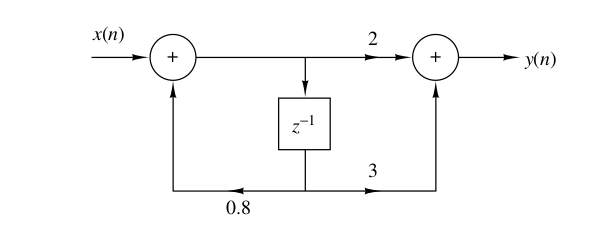
\includegraphics[width=10cm]{figures/fig49.png}
  \caption{Figure P49 from textbook}
    \label{fig:number49_fromText}
\end{figure}
\vspace{2em}
\hrule
\newpage
\section{}
2.52 - Problem 2.52 part (a). (15 points)\\
Consider the systems shown in Fig. P52.\\
\begin{figure}[ht!]
  \centering
  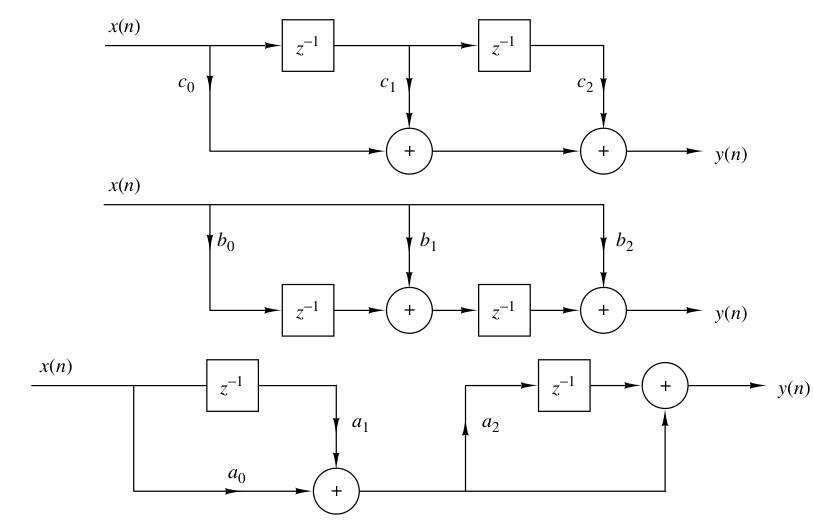
\includegraphics[width=14cm]{figures/fig52.png}
  \caption{Figure P52 from textbook}
    \label{fig:number52_fromText}
\end{figure}
\begin{enumerate}
\item Determine and sketch their impulse responses $h1 (n)$, $h2 (n)$, and $h3 (n)$.
\item Is it possible to choose the coefficients of these systems in such a way that: \center{$h_1 (n) = h_2 (n) = h_3 (n)$}
\end{enumerate}
\vspace{2em}
\hrule
\end{document}




